%%%%%%%%%%%%%%%%%%%%%%%%
%
% $Autor: Wings $
% $Datum: 2020-07-24 09:05:07Z $
% $Pfad: GDV/Vortraege/latex - Ausarbeitung/Kapitel/Einleitung.tex $
% $Version: 4732 $
%
%%%%%%%%%%%%%%%%%%%%%%%%

\chapter{Knowledge Discovery in Databases (KDD) Process}

KDD plays a pivotal role in helping organizations navigate the over whelming volumes of data generated in today’s information-driven world. KDD is a structural approach to data analysis to discover and make explicit knowledge available in extensive data sets \cite{Wings:2024}. This methodology involves a series of well-defined steps, including data selection, preprocessing, transformation and analysis, leading to the generation of actionable knowledge as shown in the figure ~\ref{KDD Process}. \cite{KDD:2000}

\begin{figure}
	\begin{center}
		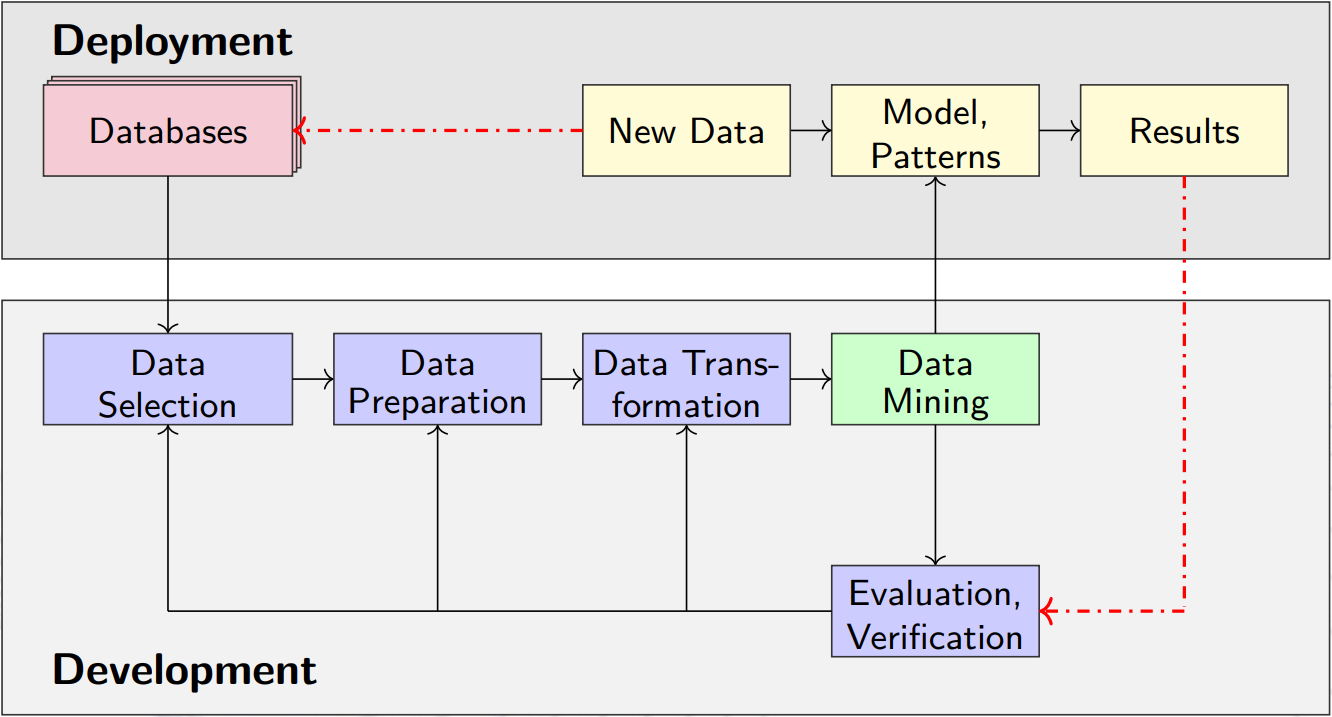
\includegraphics[width=0.7\linewidth]{Images/KDD.png}
		\caption{KDD Process}
		\label{KDD Process} 
		\cite{Wings:2024}
	\end{center}
\end{figure}

KDD is particularly relevant for analyzing log file data in the context of thread and weakness analysis. The structured approach ensures that patterns and anomalies are identified efficiently, enabling the identification of targeted solutions for improving system security and operational performance. \cite{IEEE:1997}

In this project, the KDD process will serve as the backbone for organizing and implementing analytics tasks, ensuring a systematic exploration of the data to uncover valuable insights.

\section{Topic Description}
This section of the report outlines the objective to focuses on identifying anomalies, vulnerabilities, and inefficiencies within the dataset. The primary goal is to uncover potential security risks, operational weaknesses, and performance bottlenecks through a comprehensive analysis of system logs.
The Knowledge Discovery in Databases (KDD) process was utilized to manage the complexity of the dataset effectively. This structured methodology enabled efficient data handling, cleaning and preparation. By leveraging the KDD process, the analysis distinguished patterns indicative of normal and abnormal behavior, identified clusters of high-risk events based on suspicious trace of useragents.
By combining statistical techniques, machine learning algorithms, and domain expertise, the analysis contributed significantly to the overall enhancement of system monitoring and management.

\subsection{Special Challenges}

\begin{itemize}
	\item The challenges in this dataset includes efficiently handling the high volume of log entries.
	\item  Additionally, the dataset used in this project was not labeled, which posed difficulties for supervised analysis.
	\item Another challenge was that log entries were not sequentially arranged by \SHELL{TraceId}, as logs are ordered by timestamp due to concurrent requests. Grouping and organizing requests using \SHELL{TraceId} was necessary for accurate analysis, adding complexity to preprocessing.
	
\end{itemize}

\section{Database}

The database used in this project comprised of log files collected from the system. The analysis was performed collectively on nine log files dated 20th November, 21st November, 23rd November, 24th November, 26th November, 27th November, 29th November, 30th November, and 1st December, 2024.


\section{Data Selection}

Data selection is a critical step that directly influences the project’s outcomes. It focuses on identifying relevant portions of the log files for analysis while filtering out irrelevant data to ensure only attributes contributing to the project objectives are prioritized.

\subsection{Origin}
Logs generated by monitoring tools and event management systems, specifically collected from the Graylog server.

\subsection{Data Format}
The file format is \FILE{.log}.

\subsection{Features}
The dataset includes log entries with the following attributes
	\begin{itemize}
	\item Timestamps
	\item PID
	\item Logger
	\item Message
	\item Scope (e.g., TraceId, RequestID)
	\item Application
	\item State
	\item EventID
\end{itemize}

\subsection{Size}
The dataset is approximately 3.34 GB size.

\section{Data Preparation}
Data preparation in the Knowledge Discovery in Databases (KDD) process, ensures the dataset is clean, consistent and ready for analysis. 

\subsection{Merging and Conversion}
\begin{itemize}
	\item The initial step involved merging all nine individual log files into a single consolidated file. 
	\item Then the merged file, originally in format \FILE{.log}, were converted to CSV file to facilitate easier manipulation as shown in the figure ~\ref{csvFile}.
\end{itemize}

\begin{figure}
	\begin{center}
		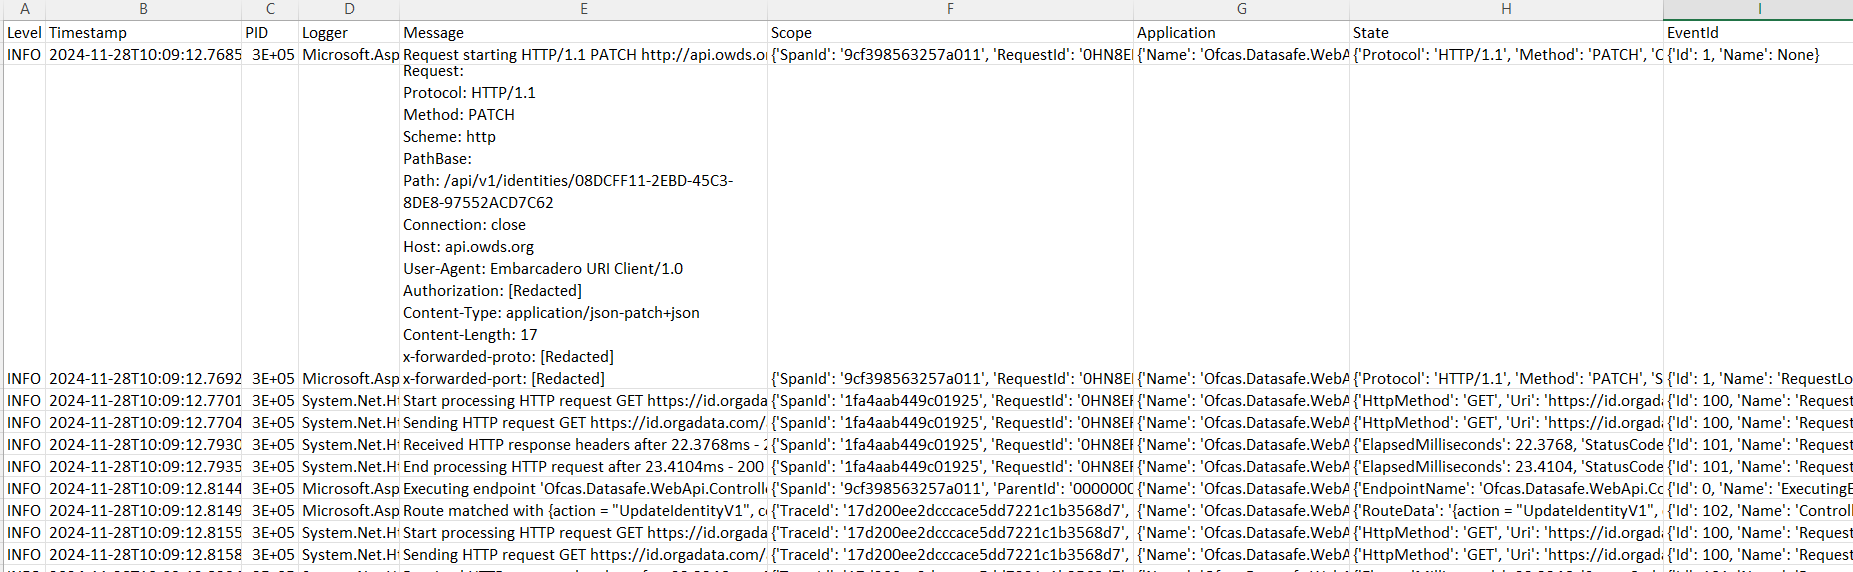
\includegraphics[width=0.9\linewidth]{Images/csvFile.png}
		\caption{Converted CSV file}
		\label{csvFile} 
	\end{center}
\end{figure}

\subsection{Initial Cleaning}
\begin{itemize} 
	\item Excluding entries without a valid TraceId that contain generic error or warning messages as shown in figure ~\ref{error}.
\end{itemize}
\begin{figure}
	\begin{center}
		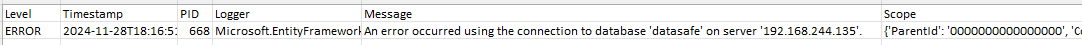
\includegraphics[width=0.9\linewidth]{Images/error.png}
		\caption{Error log}
		\label{error} 
	\end{center}
\end{figure}

\subsection{Key Attributes}
The following were the key parameters that were identified and prioritized for analysis,
\begin{itemize}
	\item \SHELL{TraceId}: Used to track individual requests across log entries, enabling the grouping and analysis of entire request flows.
	\item \SHELL{HTTP Status Code}: Identifies the result of a request (e.g., success, client errors, or server errors). Codes such as 200, 404 and 500 provide critical insights into system health.
	\item \SHELL{Path}: Represents the API endpoint or resource accessed during a request, useful for pinpointing affected components or services.
	\item \SHELL{User-Agent}: Provides details about the client or system making the request, helping to identify trends in usage or unusual activity from specific sources.
\end{itemize}

\section{Data Transformation}

This section focuses on manipulating and reshaping the cleaned data into a structured format ready for analysis. The key transformation includes,

\begin{enumerate}
	\item Grouping log entries by \SHELL{TraceId} to reconstruct complete request flows.
	\item Parsing relevant fields (\SHELL{TraceId, HTTP Status Code, Path, User-Agent}) from JSON structures.
	\item Transforming each row to represent a unique log entry with all associated fields (e.g., aligning \SHELL{TraceId} with its corresponding attributes) as shown in figure ~\ref{DataTrans}.
\end{enumerate}

\begin{figure}
	\begin{center}
		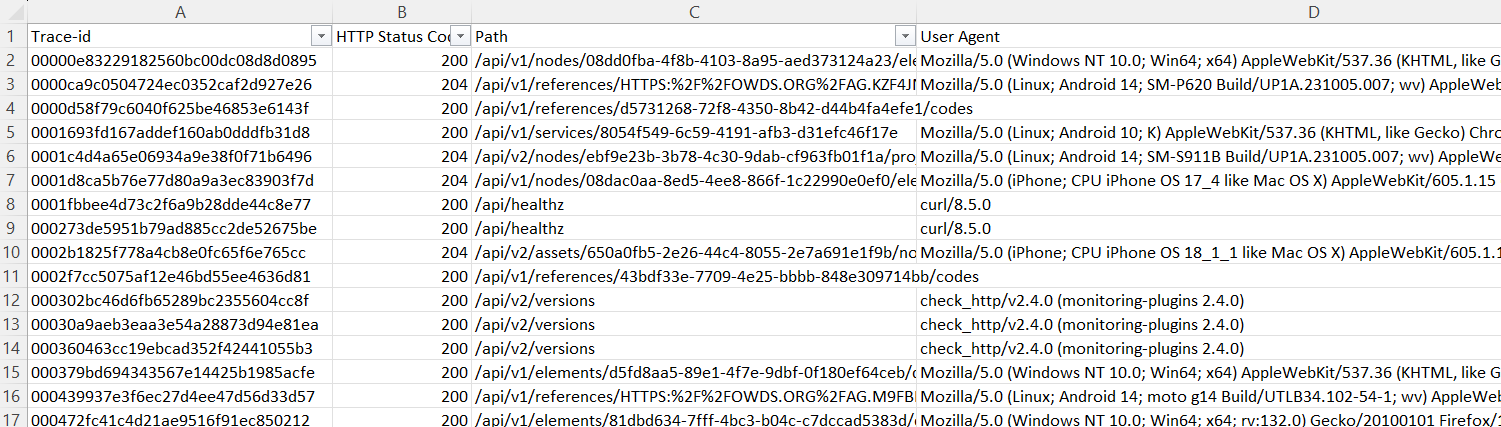
\includegraphics[width=0.9\linewidth]{Images/DataTransformation.png}
		\caption{Result after applying data transformation}
		\label{DataTrans} 
	\end{center}
\end{figure}

\section{Data Mining}
Data mining involves extracting hidden patterns and anomalies from datasets. In this project, clustering and anomaly detection were utilized to uncover system irregularities and potential security threats efficiently.
\subsection{Feature Extraction}
Feature extraction involves converting raw data into a format that can be processed by machine learning algorithms.
\begin{itemize}
	\item In this project, TF-IDF (Term Frequency-Inverse Document Frequency) Vectorization technique is used, to convert textual data (like the Path attribute in the log data) into numerical features. This allows the model to understand which paths are accessed frequently and which are less common, making it easier to identify unusual patterns.
	\item TF-IDF vectors were combined with additional numeric attributes such as HTTP status codes, unique paths and user-agents.
\end{itemize}

\subsection{Clustering}
Clustering was performed using DBSCAN (Density-Based Spatial Clustering of Applications with Noise):
\begin{itemize}
	\item DBSCAN groups requests that shared similar patterns, such as accessing the same paths with similar HTTP Status Codes and User-Agents were grouped into clusters.
	\item Requests that did not belong to any cluster were flagged as anomalies (DBSCAN\_Cluster = -1).
\end{itemize}

\subsection{Anormalities}
Along with clustering, Anomaly detection focuses on identifying unusual behaviors that deviate significantly from the norm using Isolation forest.
\begin{itemize}
	\item The model analyzed the combined features (TF-IDF vectors and numeric attributes) to detect anomalous requests.
	\item By integrating DBSCAN and Isolation Forest approach, robust anomaly detection was ensured through both density-based and statistical methods.
\end{itemize}


\section{Model}
The model selection was driven by the need to perform both clustering and anomaly detection effectively. A combination of unsupervised and ensemble-based learning techniques was employed to analyze request patterns and identify anomalies.

\subsection{DBSCAN}
DBSCAN is a density-based clustering algorithm, groups data points that are closely packed together based on a density threshold. Data points far from any dense cluster are treated as "noise" or anomalies.
\subsubsection{Key Parameters}
\begin{itemize}
	\item \textbf{eps}: Set to 0.5, defining the maximum distance between points to form a cluster.
	\item \textbf{min\_samples}: Set to 5, specifying the minimum number of points required to form a cluster.
\end{itemize}
\subsubsection{Outcome}
Requests not assigned to any cluster (cluster = -1) were flagged as anomalies.

\subsection{Isolation Forest}
Isolation Forest is an ensemble learning technique designed to detect outliers by isolating data points. It works on the principle that anomalies are easier to isolate because they have unique features.
\subsubsection{Key Parameters}
\begin{itemize}
	\item \textbf{n\_estimators:} Set to 100, specifying the number of decision trees.
	\item \textbf{contamination:} Set to 0.01, indicating the proportion of expected anomalies in the dataset.
	\item \textbf{random\_state:} Ensured reproducibility of results with a fixed seed value (42).
\end{itemize}
\subsubsection{Outcome}
Requests identified as anomalies were flagged with a value of -1.

\section{Validation/Verification}
Validation and verification are critical steps to ensure the reliability and accuracy of the data mining and anomaly detection process. This section outlines the methods used to validate the models and verify the results.

\subsection{DBSCAN Validation}
The results of the DBSCAN clustering were validated as follows:
\begin{itemize}
	\item The clustering results were reviewed to ensure that data points in the same cluster exhibited similar patterns.
	\item Anomalies (\texttt{Cluster = -1}) were manually inspected to confirm that they represented requests deviating from normal patterns.
\end{itemize}

\subsection{Isolation Forest Validation}
The Isolation Forest model's performance was validated using the following methods:
\begin{itemize}
	\item \textbf{Anomaly Score Distribution}: The distribution of anomaly scores was evaluated to differentiate anomalies from regular requests.
	\item \textbf{Manual Inspection}: A subset of flagged anomalies was reviewed to confirm their unusual characteristics.
\end{itemize}

\section{Data Visualization}

\section{Conclusion}

